\documentclass{beamer}
\usepackage{minted}
\usemintedstyle{manni}
\usepackage{hyperref}
\hypersetup{
colorlinks=true,
urlcolor=blue
}
\usepackage{graphicx}

\begin{document}
\title{Securing Django Websites}
\author{Nick Thompson} 
\date{\today}

\frame{\titlepage}

\begin{frame}[fragile]
\frametitle{Getting started:}
\begin{minted}{bash}
$ git clone https://github.com/NAThompson/django_https.git
$ pyvenv django_https
$ cd django_https
$ sudo /bin/bash
# pip3 install -r requirements.txt
# . bin/activate
\end{minted}
\end{frame}

\begin{frame}
\frametitle{Server Stack}
\begin{itemize}
\item We're going to use Django+gunicorn+nginx to serve this website
\item \href{http://gunicorn.org/\#deployment}{gunicorn} is a web server gateway interface
\item We need nginx to reverse proxy because gunicorn is trivially vunerable to DOS attacks
\end{itemize}
\end{frame}

\begin{frame}[fragile]
\frametitle{Install nginx}
\begin{minted}{bash}
$ sudo apt-get install nginx # Ubuntu
$ sudo brew install nginx # Mac
\end{minted}
\end{frame}

\begin{frame}[fragile]
\frametitle{Symlink our nginx.conf into the global}
\begin{minted}{bash}
$ cd django_https
$ rm -f /etc/nginx/nginx.conf /etc/nginx/sites-available/default
$ ln -s `pwd`/nginx.conf /etc/nginx/nginx.conf
$ ln -s `pwd`/default /etc/nginx/sites-available/default
\end{minted}
(Sorry peeps I didn't bother to relativize all the paths; you'll need to edit!)
\end{frame}

\begin{frame}[fragile]
Now we can serve the website:
\begin{minted}{bash}
django_https/src# gunicorn -c gunicorn_config.py https.wsgi &
django_https/src# nginx
\end{minted}
Again, there are some hard-coded paths in there you'll need to edit . . .
\end{frame}

\begin{frame}[fragile]
\frametitle{Redirects}
If we don't listen on port 80, then users will need to type the protocol into the browser, which no one does. 

Hence we need nginx to redirect:
\begin{minted}{c}
server {
       listen         80;
       listen         [::]:80;
       server_name    www.example.com example.com;
       return         301 https://$server_name$request_uri;
}
\end{minted}
\end{frame}

\begin{frame}[fragile]
\frametitle{Turn SSL on and proxy-pass to gunicorn}
\begin{minted}{c}
server {
       listen         443;
       ssl            on;
       server_name    example.com;
       ssl_certificate  example.com/bundle.crt;
       ssl_certificate_key example.com.key;

       location / {
             proxy_pass https://127.0.0.1:8000;
             proxy_set_header Host $host;
             proxy_set_header X-Forwarded-For $proxy_add_x_forwarded_for;
       }
}
\end{minted}
\end{frame}

\begin{frame}[fragile]
\frametitle{How secure is the default nginx configuration?}
\href{https://www.ssllabs.com/ssltest/analyze.html}{SSL Labs} doesn't think it's all that great:

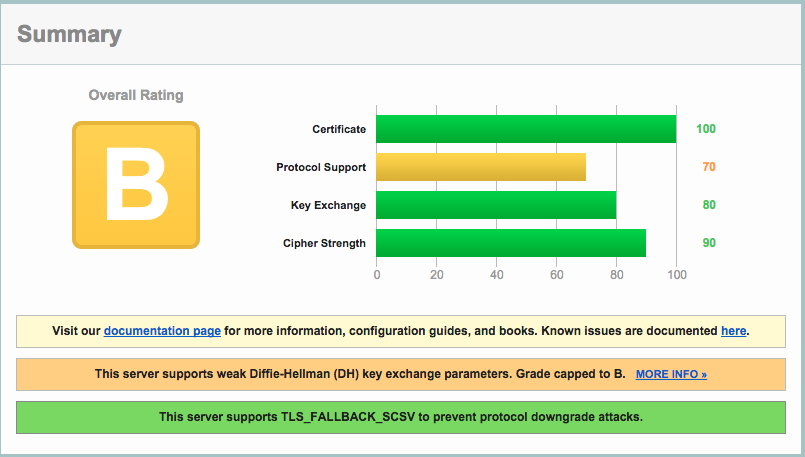
\includegraphics[scale=0.25]{figures/SSLLabsFirstGrade.png}
\end{frame}

\begin{frame}[fragile]
\frametitle{Improving SSLLabs grade}
In the nginx.conf, change 
\begin{minted}{c}
ssl_protocols TLSv1 TLSv1.1 TLSv1.2;
\end{minted}
to
\begin{minted}{c}
ssl_protocols TLSv1.2;
\end{minted}
Note: This will lose you some old IE browsers. SSLLabs will tell you which ones on their report.
\end{frame}

\begin{frame}[fragile]
\frametitle{Improving SSLLabs grade}
SSLLabs thinks that 256 bits symmetric protocols are better than 128 bit protocols, so we need to restrict the supported ciphers:
\begin{minted}{c}
ssl_ciphers 'ECDHE-RSA-AES256-GCM-SHA384:ECDHE-ECDSA-AES256-GCM-SHA384:ECDHE-RSA\
-AES256-SHA384:ECDHE-ECDSA-AES256-SHA384:ECDHE-RSA-AES256-SHA:ECDHE-ECDSA-AES256-SHA:DHE\
-RSA-AES256-GCM-SHA384:DHE-RSA-AES256-GCM-SHA:DHE-RSA-AES256-SHA256:DHE-RSA-AES256-SHA:!\
aNULL:!eNULL:!LOW:!3DES:!MD5:!EXP:!PSK:!SRP:!DSS';
\end{minted}
\end{frame}

\begin{frame}[fragile]
Now we need to get strong Diffie-Helman keys:
\begin{minted}{bash}
openssl dhparam -out dhparam.pem 4096
\end{minted}
and add it to the nginx.conf:
\begin{minted}{c}
ssl_dhparam /path_to_pem/dhparam.pem
\end{minted}
\end{frame}

\begin{frame}[fragile]
\frametitle{SSLLabs is now Happy}
\begin{figure}
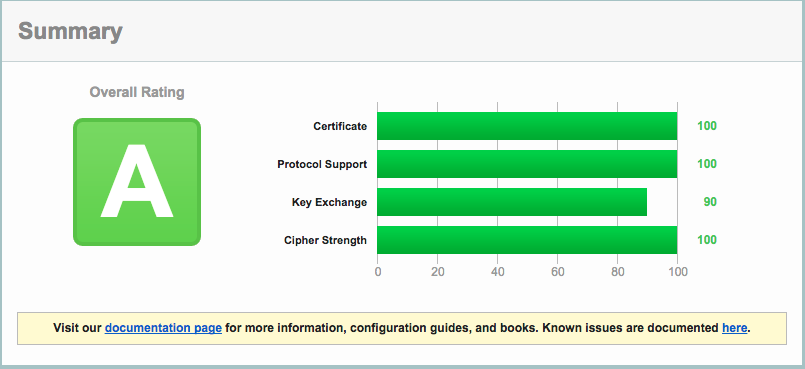
\includegraphics[scale=0.25]{figures/SSLLabsA.png}
\end{figure}
You can see the SSLLabs rating guide \href{https://www.ssllabs.com/downloads/SSL_Server_Rating_Guide.pdf}{here}.
\end{frame}



\end{document}
